\documentclass[12ptr]{article}
\usepackage[a4paper,width=150mm,headheight=110pt,top=25mm,bottom=25mm]{geometry}
\usepackage[utf8]{inputenc}
\usepackage{listings}
\usepackage{graphicx}
\usepackage{pgffor} 
\usepackage{float}
\usepackage{graphics} 
\usepackage{fancyhdr}
\usepackage{titling}
\usepackage{hyperref}
\usepackage{caption}
\usepackage{subfig}

%\renewcommand\maketitlehooka{\null\mbox{}\vfill}
%\renewcommand\maketitlehookd{\vfill\null}


%----------------------------------------------------------------------------------------
%	Title Page
%---------------------------------------------------------------------------------------
\begin{document}

\vspace*{5cm}
 \begin{center}
{\huge \bf GPU Computing for Bionanotechnology}\\[0.2cm]
{\large \bf Mentor: Prof. Aleksei Aksimentiev}\\[0.2cm]
{\large Mentee: Swan Htun (SPIN)}\\[0.2cm]
{July 23 2019}\\[0.5cm]
\end{center}

\begin{figure}[!ht]
    \centering
    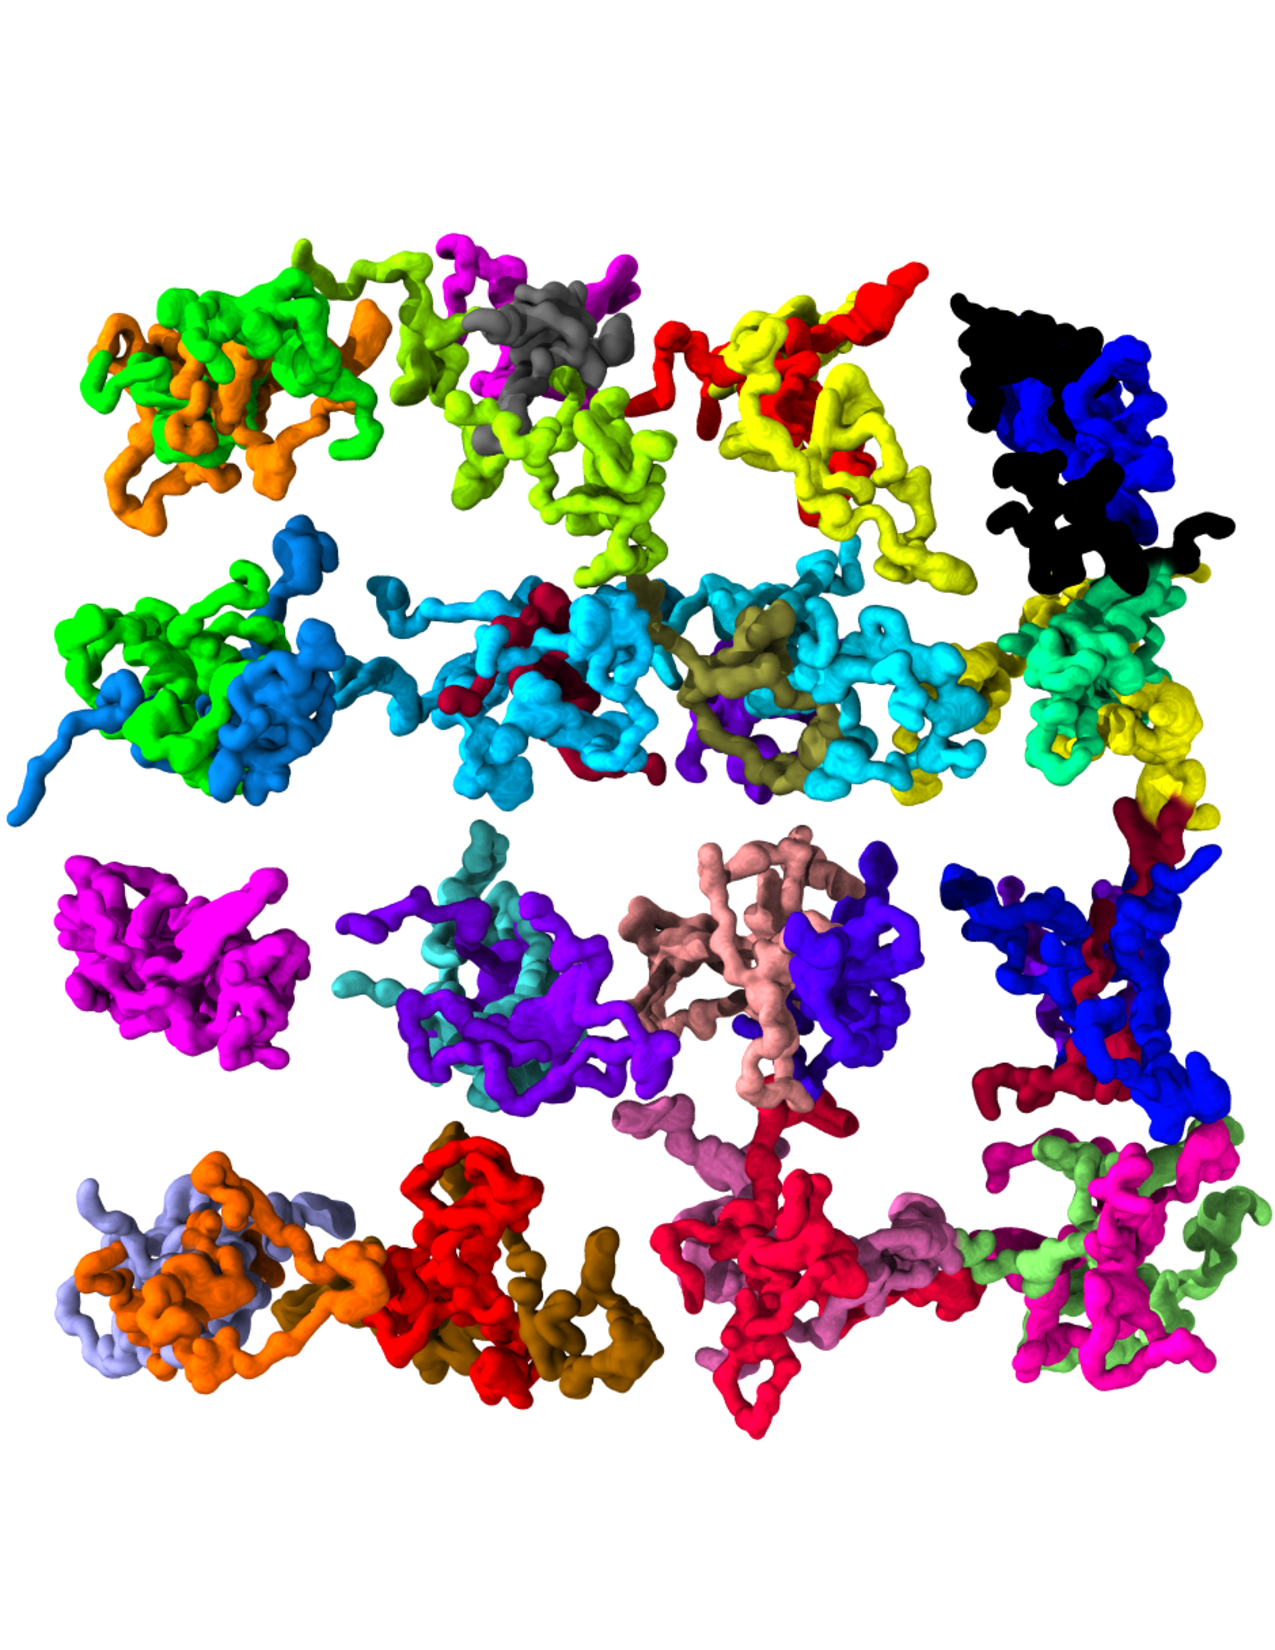
\includegraphics[width=6cm]{fus400_64_first.pdf}
    \qquad
    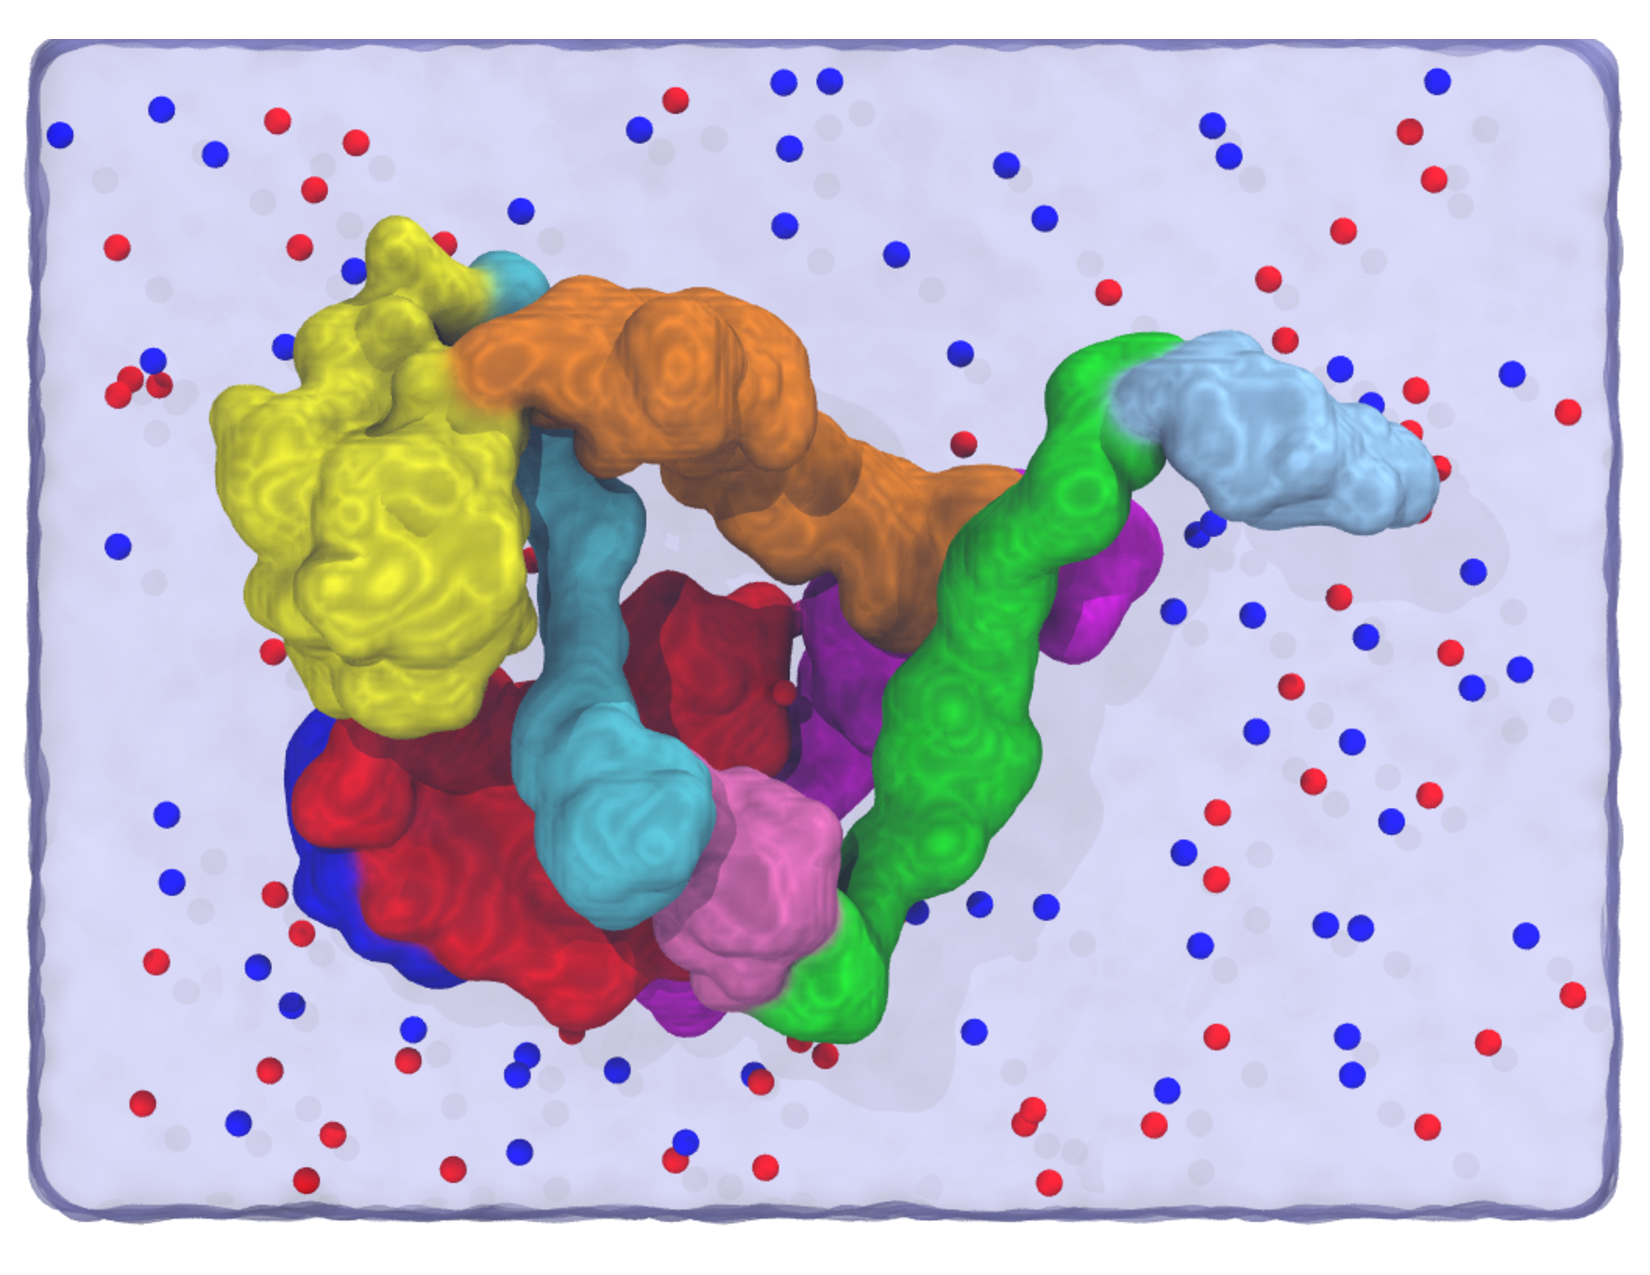
\includegraphics[width=7cm]{all_atom_fus1.pdf} 
\end{figure}


\newpage


%----------------------------------------------------------------------------------------
%	Table of Contents
%---------------------------------------------------------------------------------------
%\addtocontents{toc}{\setcounter{tocdepth}{1}} % Set depth to 1
\tableofcontents
\newpage

\section{Abstract}
Fused in Sarcoma (FUS) is a RNA-binding protein involved in various cellular processes such as DNA repair, RNA transport and damage response \cite{Patel_15}. It undergoes liquid-liquid phase separation (LLPS) process and displays liquid-like properties \cite{Patel_15}. In this study, we investigate various conditions that affects phase separation process of both wild-type (WT) and mutant FUS protein, such as temperature and concentration using computational approaches. The results of the Brownian Dynamic simulations run at various temperatures ranging from $295K$ to $450K$ suggest that phase transition occurs around $415K$. Further simulations at different concentrations are being carried out to quantify the effects of concentration in phase separation process as well as how certain mutations interfere with phase transitions of FUS. 

\section{Introduction}

Biological cells have compartmentalized cellular space for efficient regulation of biochemical reac-tions by isolating certain biochemical process from the rest of the cell by bounding the reactions inside membraneous organelles. Eukaryotic cells, however, also have many organelles that lack membrane-enclosed structures \cite{Mullard_19}, such as stress granules, and nucleoli \cite{Mullard_19}. Such membraneless organelles are commonly known as biomolecular condensates \cite{Banani_17}. Due to their highly dynamic nature, they have liquid-like properties and are formed via liquid-liquid phase separation (LLPS) process as a response to specific biochemical signals \cite{Banani_17}. Such properties include the rapid exchange of their constituent molecules with the surrounding cytoplasm or nucleoplasm \cite{Mullard_19} as well as the ability to deform and freely flow around surfaces of other intracellular structures while under shear stress \cite{Banani_17}. They also undergo fusion and fission \cite{Patel_15, Mullard_19, Banani_17}.\\[0.01cm]

These condensates have specific macromolecular composition that can be classified qualitatively into two types: clients, which are preferentially recruited as part of the condensate, and scaffolds, which are required for the formation of the condensate. The majority of the condensate is comprised of clients \cite{Banani_17}.\\[0.01cm]

The properties and molecular mechanism of these biological condensates have become an interesting topic of research, specifically intrinsically disordered proteins like FUS, as growing evidence suggests their implication in pathogenesis of amyotrophic lateral sclerosis (ALS) and frontotemporal dementia (FTD) \cite{Deng_14}. Physical process involved in biomolecular condensate formation (i.e, phase separation) and certain biomolecules involved are both known, but precise molecular mechanism of formation and its related processes are still unknown. Thus, it’s still a challenge to relate specific features and properties of the condensates with the corresponding biological function, which is essential to understanding how aberrations in them contribute to disease. \\[0.01cm]

In this research paper, we begin by simulating the behavior of wild-type FUS protein to understand how it undergoes LLPS. The motivation behind the use of computational approach owes it to the challenges in determining the structural properties of the phase separated protein assemblies and in the selection of the appropriate mutations \cite{Best_18}.\\[0.01cm]

\subsection{Fused in Sarcoma (FUS)}

Each individual FUS protein is made up of 526 amino acids and consists of both ordered and disordered regions that can be divided into a prion-like domain and the RNA binding domain \cite{Murray_17}. The phase separation process has been experimentally determined to be driven primarily by the interactions between tyrosine residues from prion-like domains (PLDs) and arginine residues from RNA-binding domains (RBDs) \cite{Wang_18}. The PLDs consist mainly of intrinsically disordered regions (IDRs) that are low in amino acid diversity (polar residues and aromatic residues) \cite{Wang_18}. Such domains are highly prone to aggregation and have been associated with pathogenesis of diseases such as ALS. Mutations in PLDs have been found to accelerate the conversion of the liquid-like droplets of FUS to solid-state, which is detrimental \cite{Patel_15}.

\newpage

\section{Methodology}
Aspects of phase separation process are simulated using all-atom Molecular Dynamics (MD) and Atomic Resolution Brownian Dynamics (ARBD) simulations. The molecular events are simulated at the time scale of the biological event and are too fast to resolve experimentally, which is one of the advantages of using computational methods. MD solves Newton’s equations of motion to determine the position of the particles at each time step and provides atomic level resolution while ARBD uses Langevin equations of motion to obtain the trajectory of the atoms and is coarse-grained. The output of the simulations are the trajectory and momentum of the system and then the trajectory data is analyzed to gain insight into the phase separation process. \\

\subsection{Softwares \& Applications Used}
ARBD is a GPU-enabled code that takes advantage of the processing power of the GPUs to facilitate fast simulations and achieves better computational efficiency for large systems in comparison to all-atom MD simulations. Python script is used to interact with the ARBD engine. Since the simulation of phase separation phenomena happens at a long time scale, we mainly utilize the BD simulations.
Visualizations and the all-atom model of FUS are built using the VMD software.
All-atom MD simulations are run using NAMD software on Stampede2 supercomputer.\\

We began by building a complete all-atom model of FUS protein using publicly available data of the atomic coordinates and the structural information of each ordered segment of FUS protein on Protein Data Bank: \href {http://www.rcsb.org}{http://www.rcsb.org}. As no structures are available for the disordered regions, their structures are generated from the amino acid sequence using the Avogadro software. Then, each individual segments are linked using VMD. From the all-atom model, we generate the BD system using the python script. 

\begin{figure}[!ht]
\begin{center}
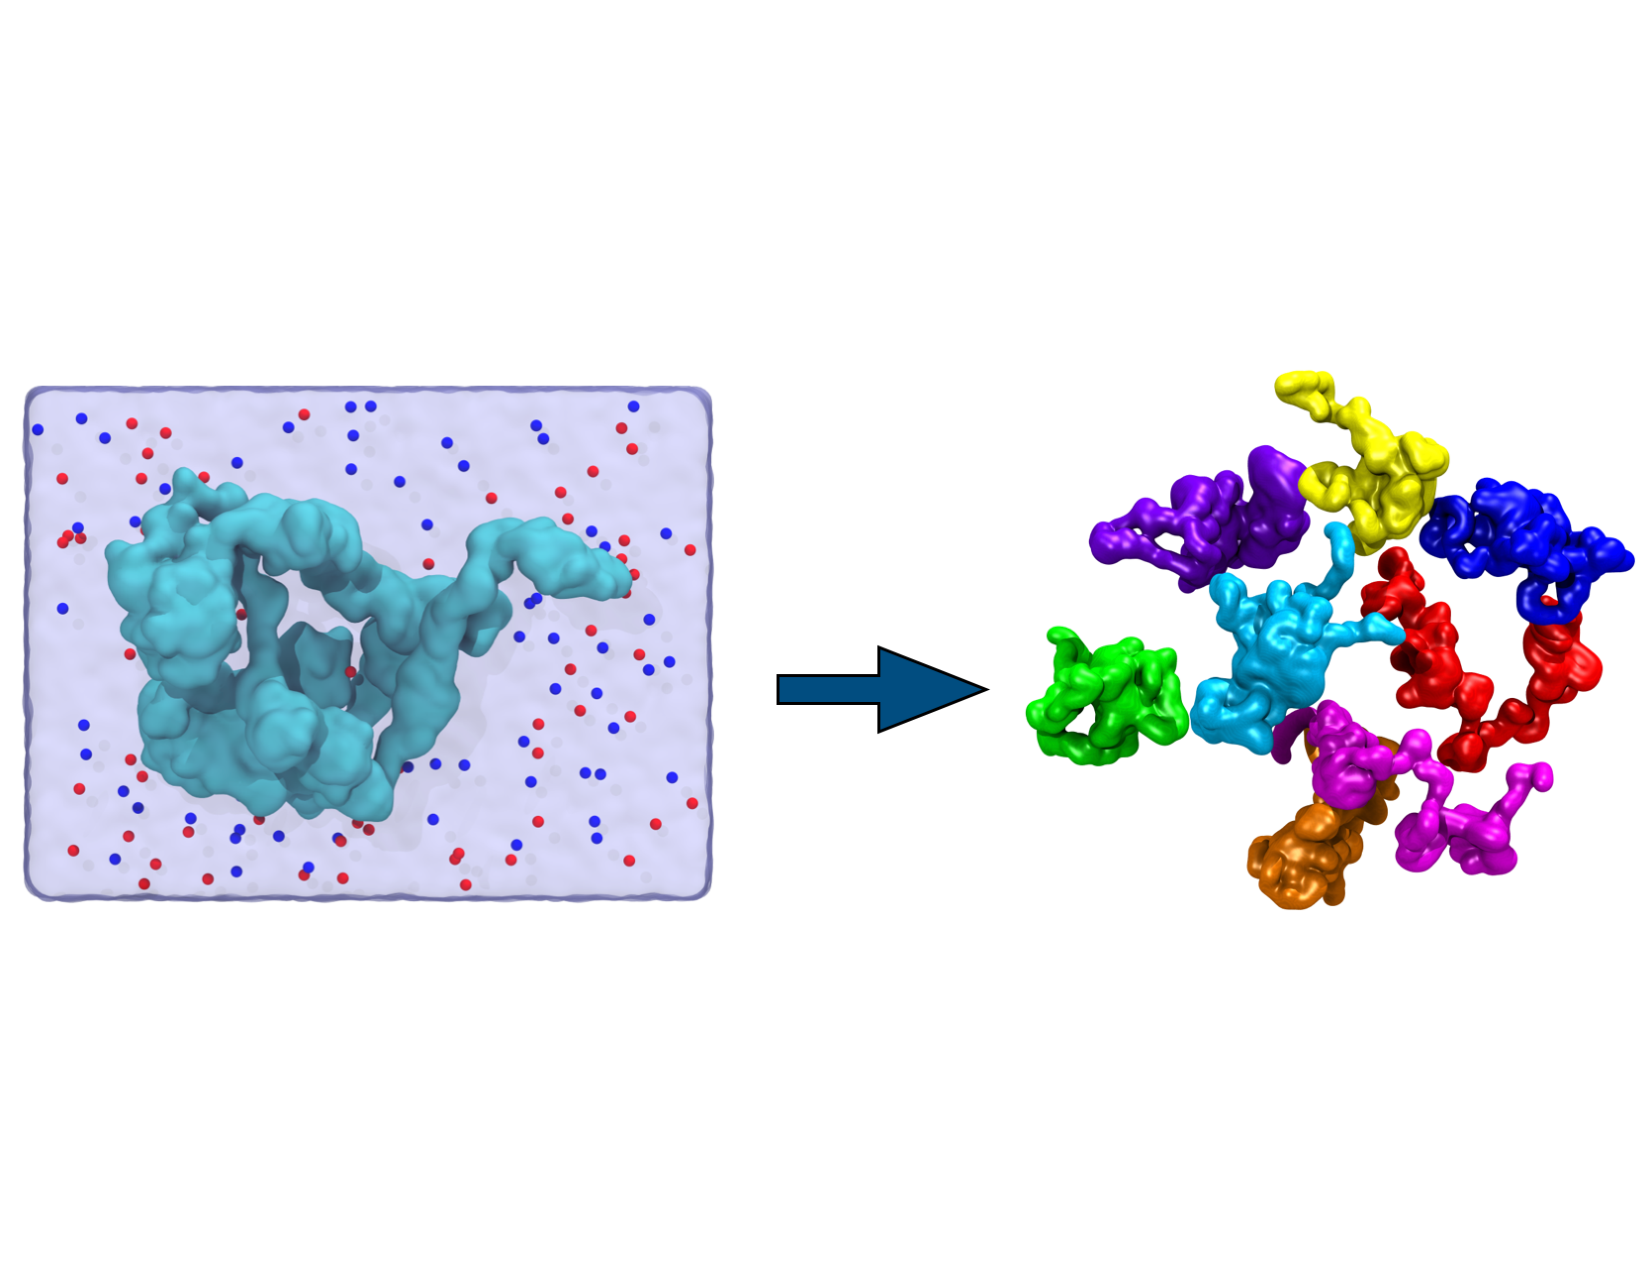
\includegraphics[width=4.0in]{all_atom_bd.pdf}
 \caption {All-atom model (left) and coarse-grain model (right) of FUS }
 \end{center}
\end{figure}

\subsection{Simulation conditions}
All-atom simulations of WT FUS protein are run at $300K$with NPT conditions. The ARBD simulations of 8 WT FUS proteins are run at $295K, 350K, 400K, 410K, 415K, 420K, 425K, 430K, 440K$ and $450K$ in NVT conditions for over 10 $\mu s$. Another set of ARBD simulations of 64 WT FUS proteins at similar temperatures are also being run to elicit the impact of concentration on phase transition. The concentration of the system can be calculated in the following way: 

\begin{equation}
 \frac{Protein \\num.}{ Avogadro's \\ num.}  * \frac{10 ^ {10}}{Dimensions ^ {3}} = \mu M
\end{equation}
\newpage


\section{Preliminary Results}
\begin{figure}[!ht]
    \centering
    \subfloat[The state of FUS protein at the start of simulation]{{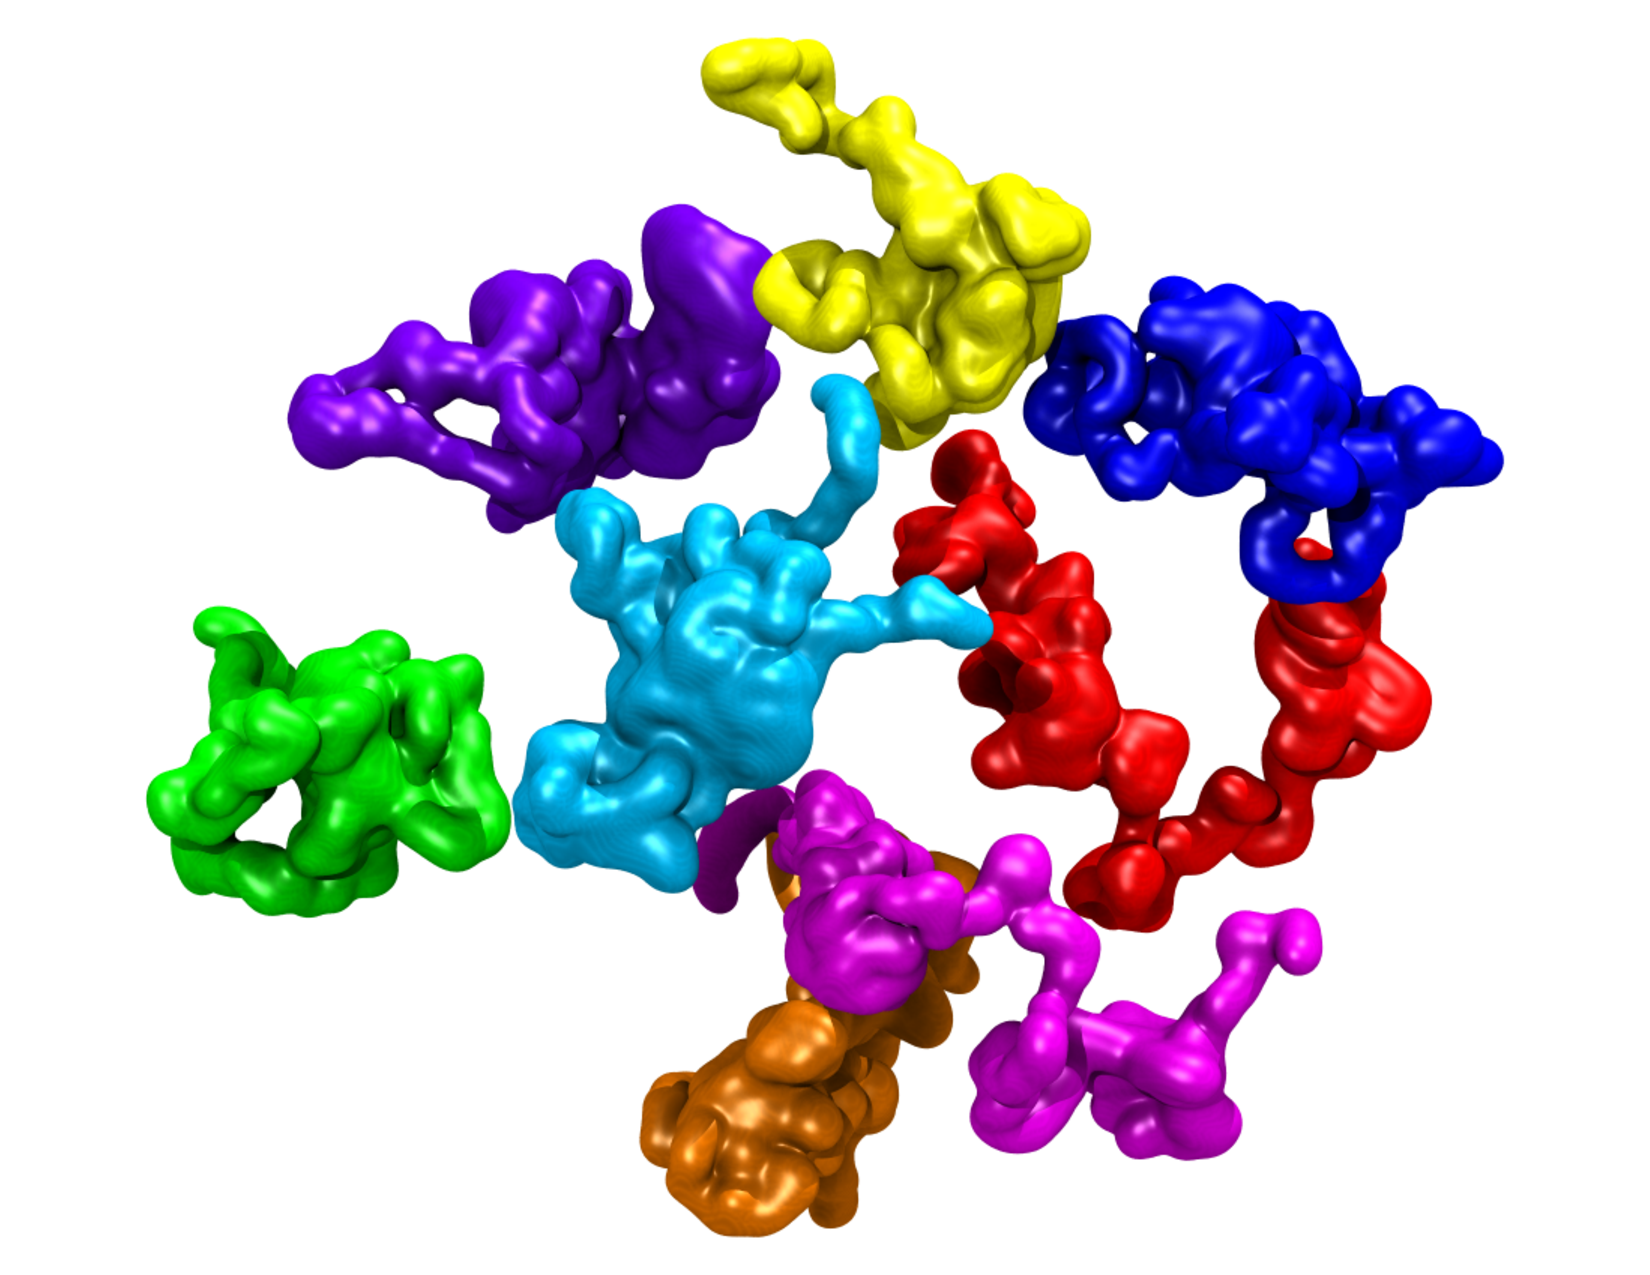
\includegraphics[width=6cm]{fus350_first.pdf} }}
    \qquad
    \subfloat[The state of FUS protein at the end of 8 $\mu s$ simulation]{{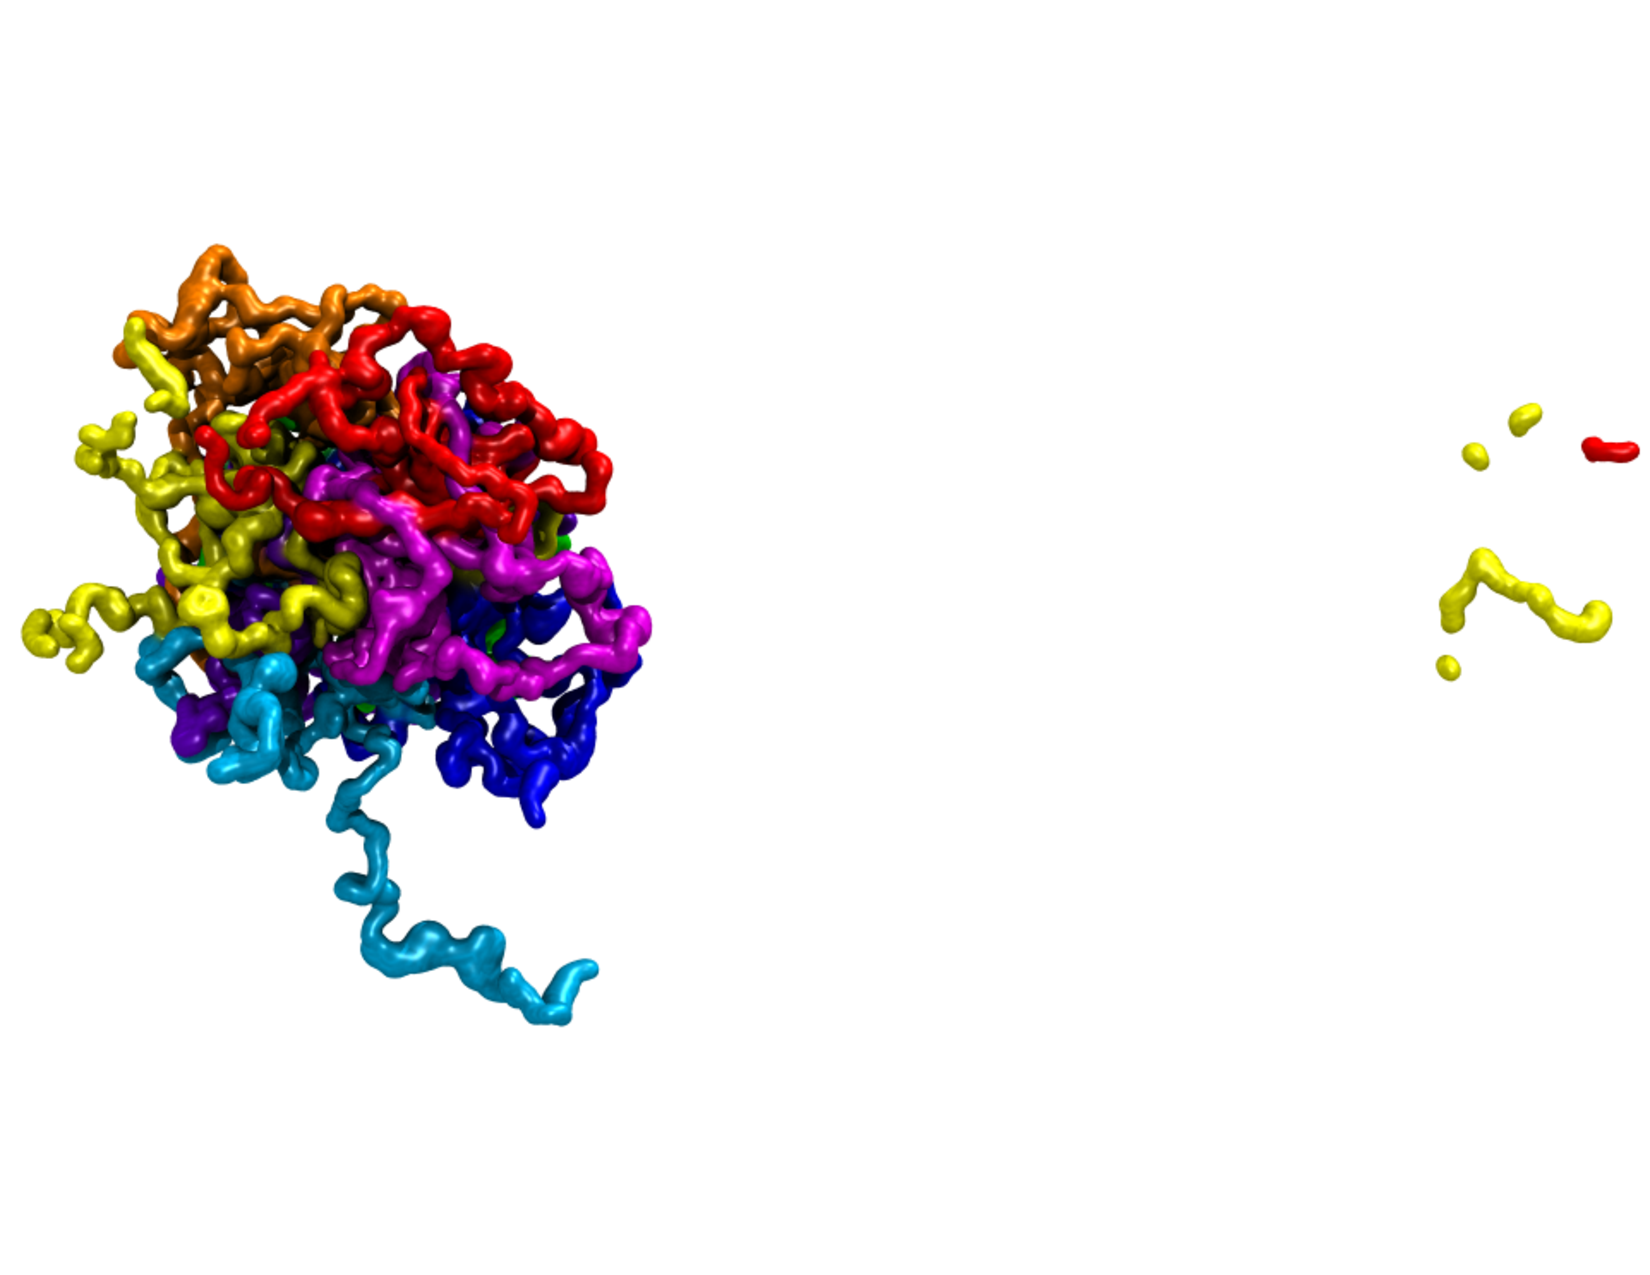
\includegraphics[width=8cm]{fus350_8_last.pdf} }}
    \caption {ARBD Simulation of FUS at 350K}
    \label{fig:fus_350}
\end{figure}

\noindent {\bf Conditions}\\
\noindent {\bf Temperature: $350K$ \\ Num. of Proteins: $8$ \\ Box volume: $825 ^{3}$ $\mathring{A} ^{3}$ \\ Concentration: $x$ \\ Total num. atoms: $4344$}
\begin{figure}[!ht]
    \centering
    \subfloat[The state of FUS protein at the start of simulation]{{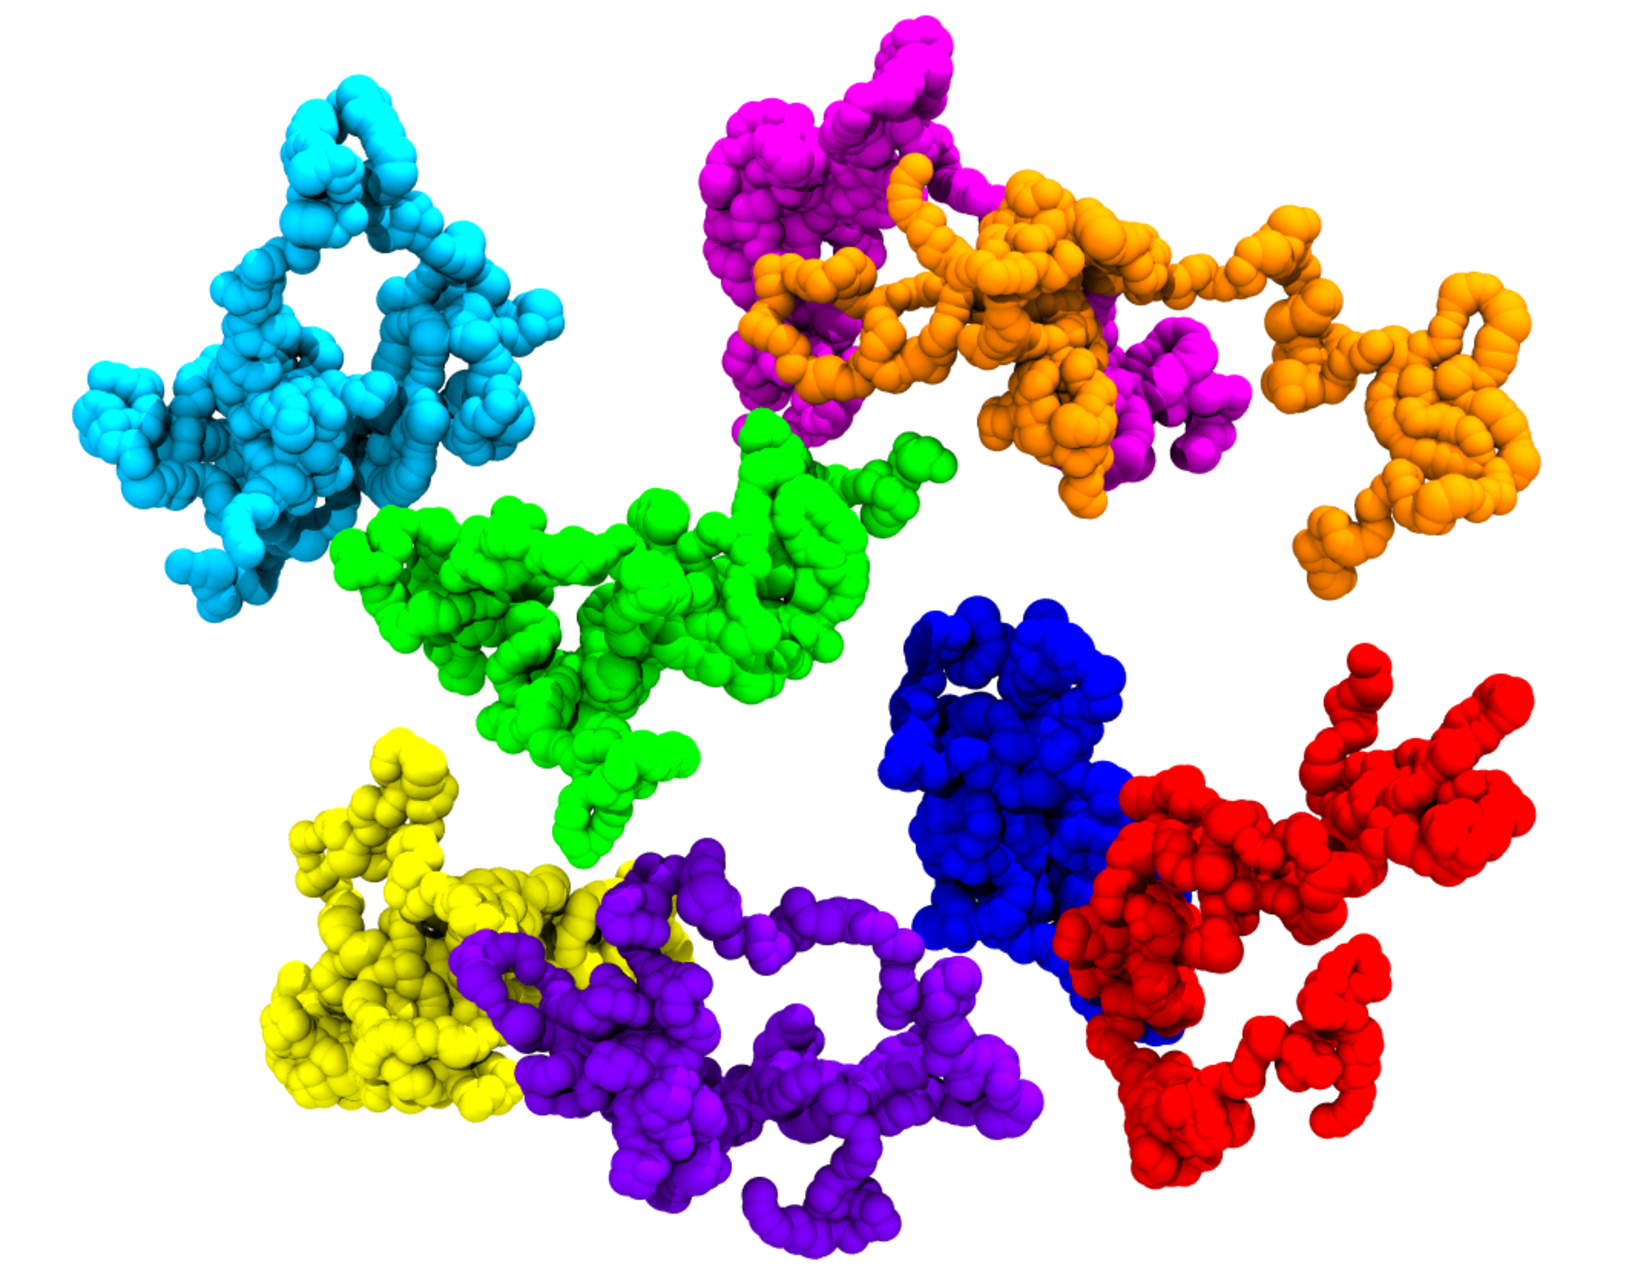
\includegraphics[width=6cm]{fus430_vdw_first.pdf} }}
    \qquad
    \subfloat[The state of FUS protein at the end of 8 $\mu s$ simulation]{{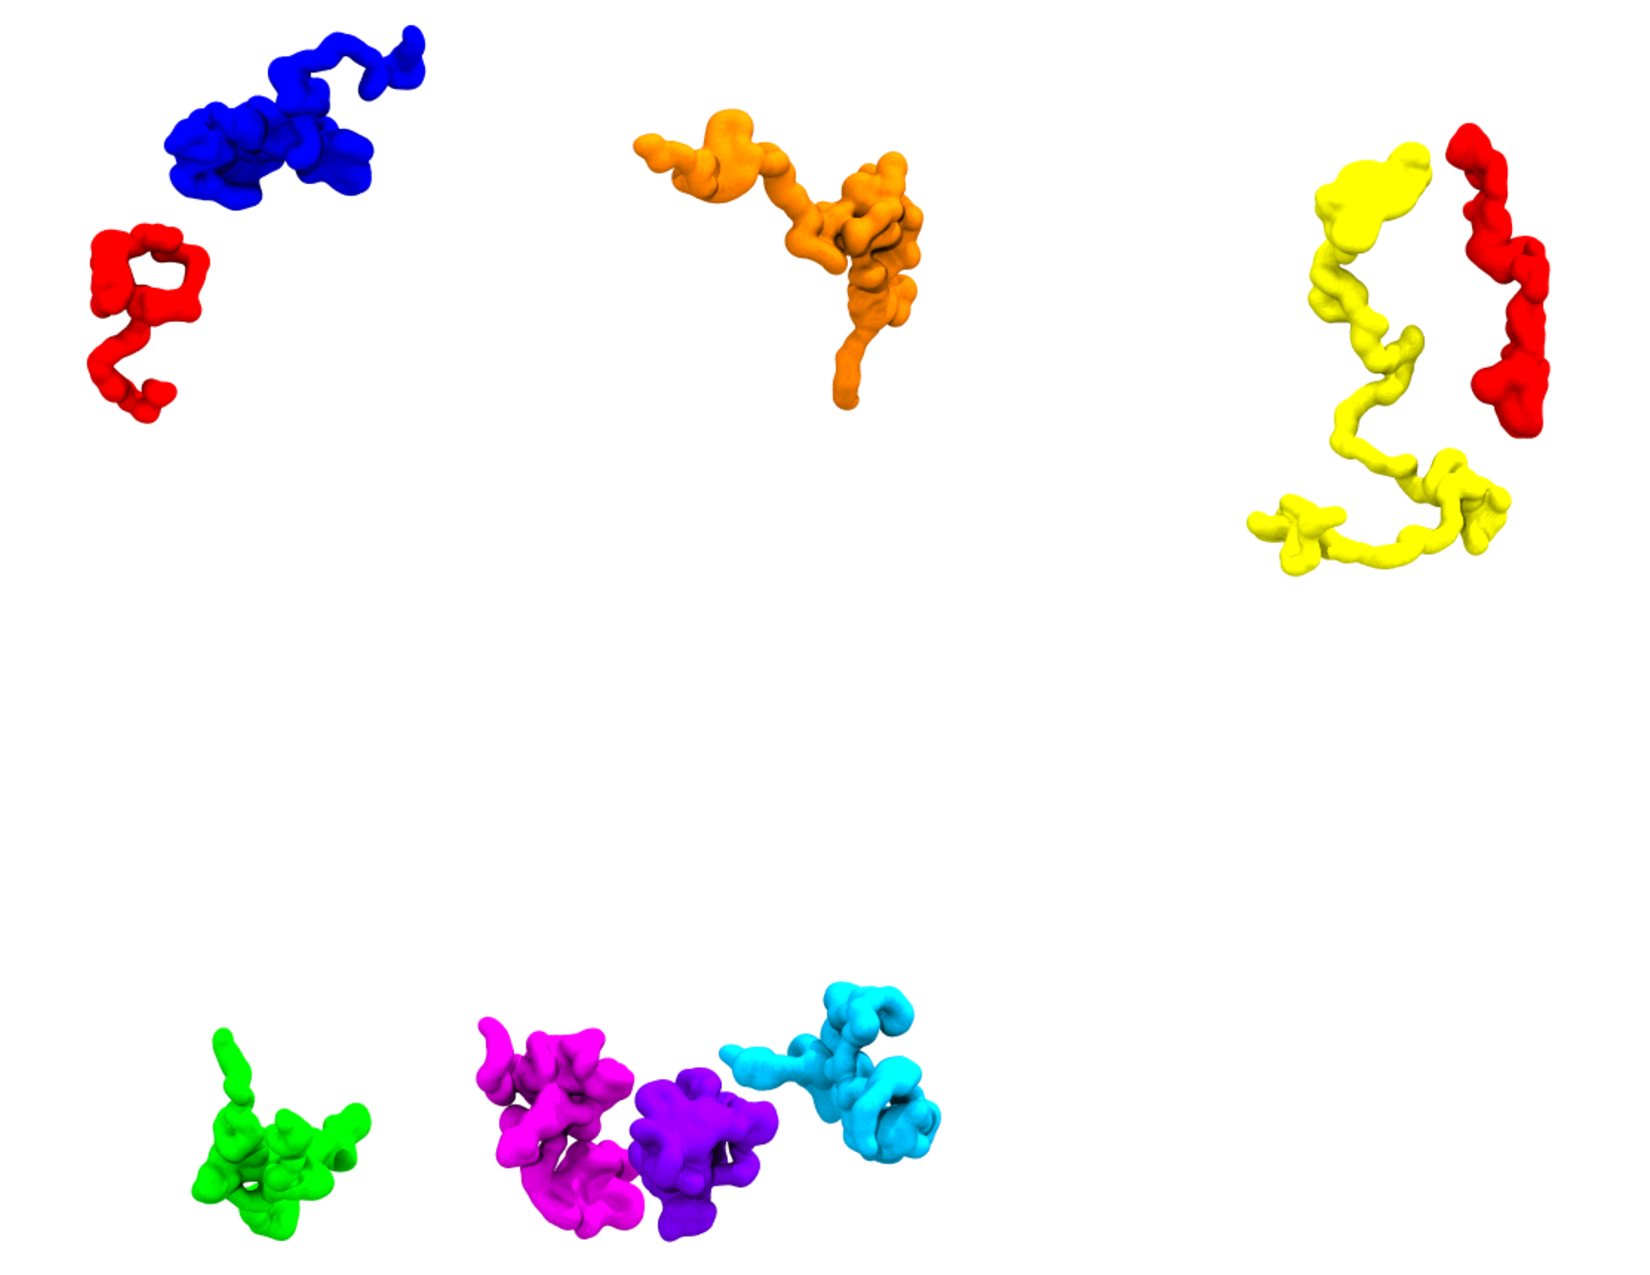
\includegraphics[width=8cm]{fus440_end.pdf} }}
    \caption {ARBD Simulation of FUS at 430K}
    \label{fig:fus_430}
\end{figure}

\noindent {\bf Conditions}\\
\noindent {\bf Temperature: $430K$ \\ Num. of Proteins: $8$ \\ Box volume: $825 ^{3}$ $\mathring{A}^{3}$ \\ Concentration: $x$ \\ Total num. atoms: $4344$}
 
\begin{figure}[!ht]
    \centering
    \subfloat[The number of contact between tyrosine and arginine residues]{{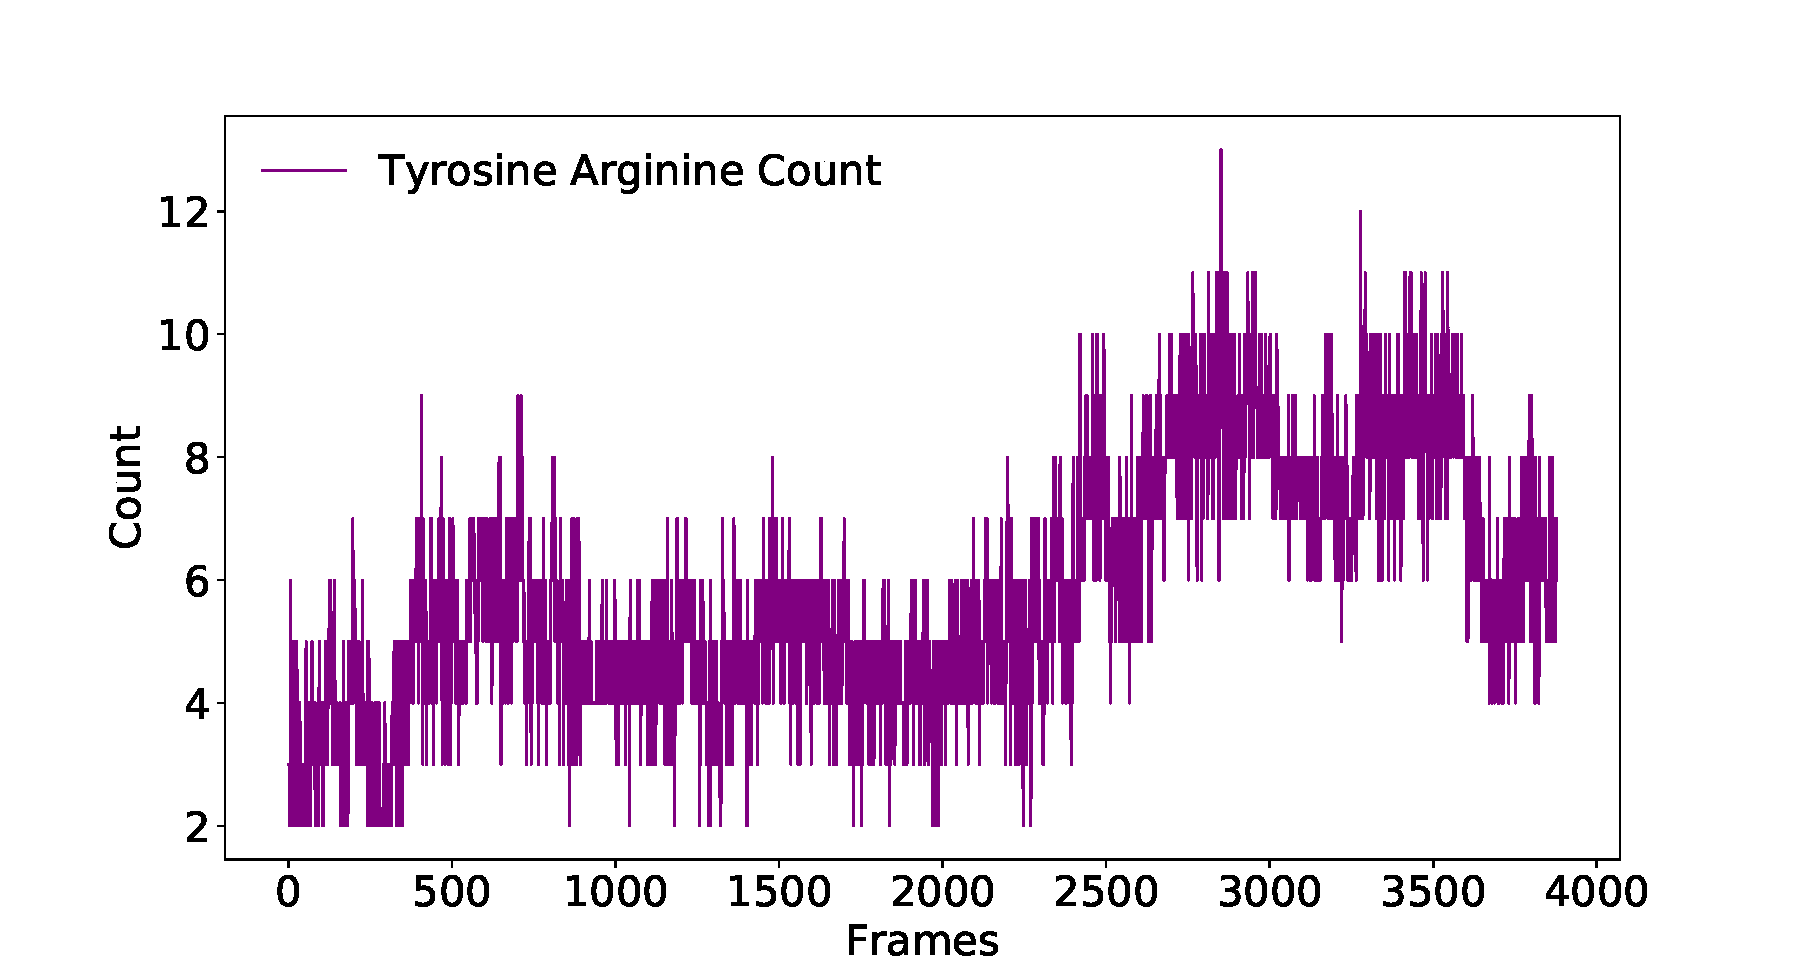
\includegraphics[width=9cm]{count_contact.pdf} }}
    \qquad
    \subfloat[Graphical representation of tyrosine and arginine residues of FUS protein]{{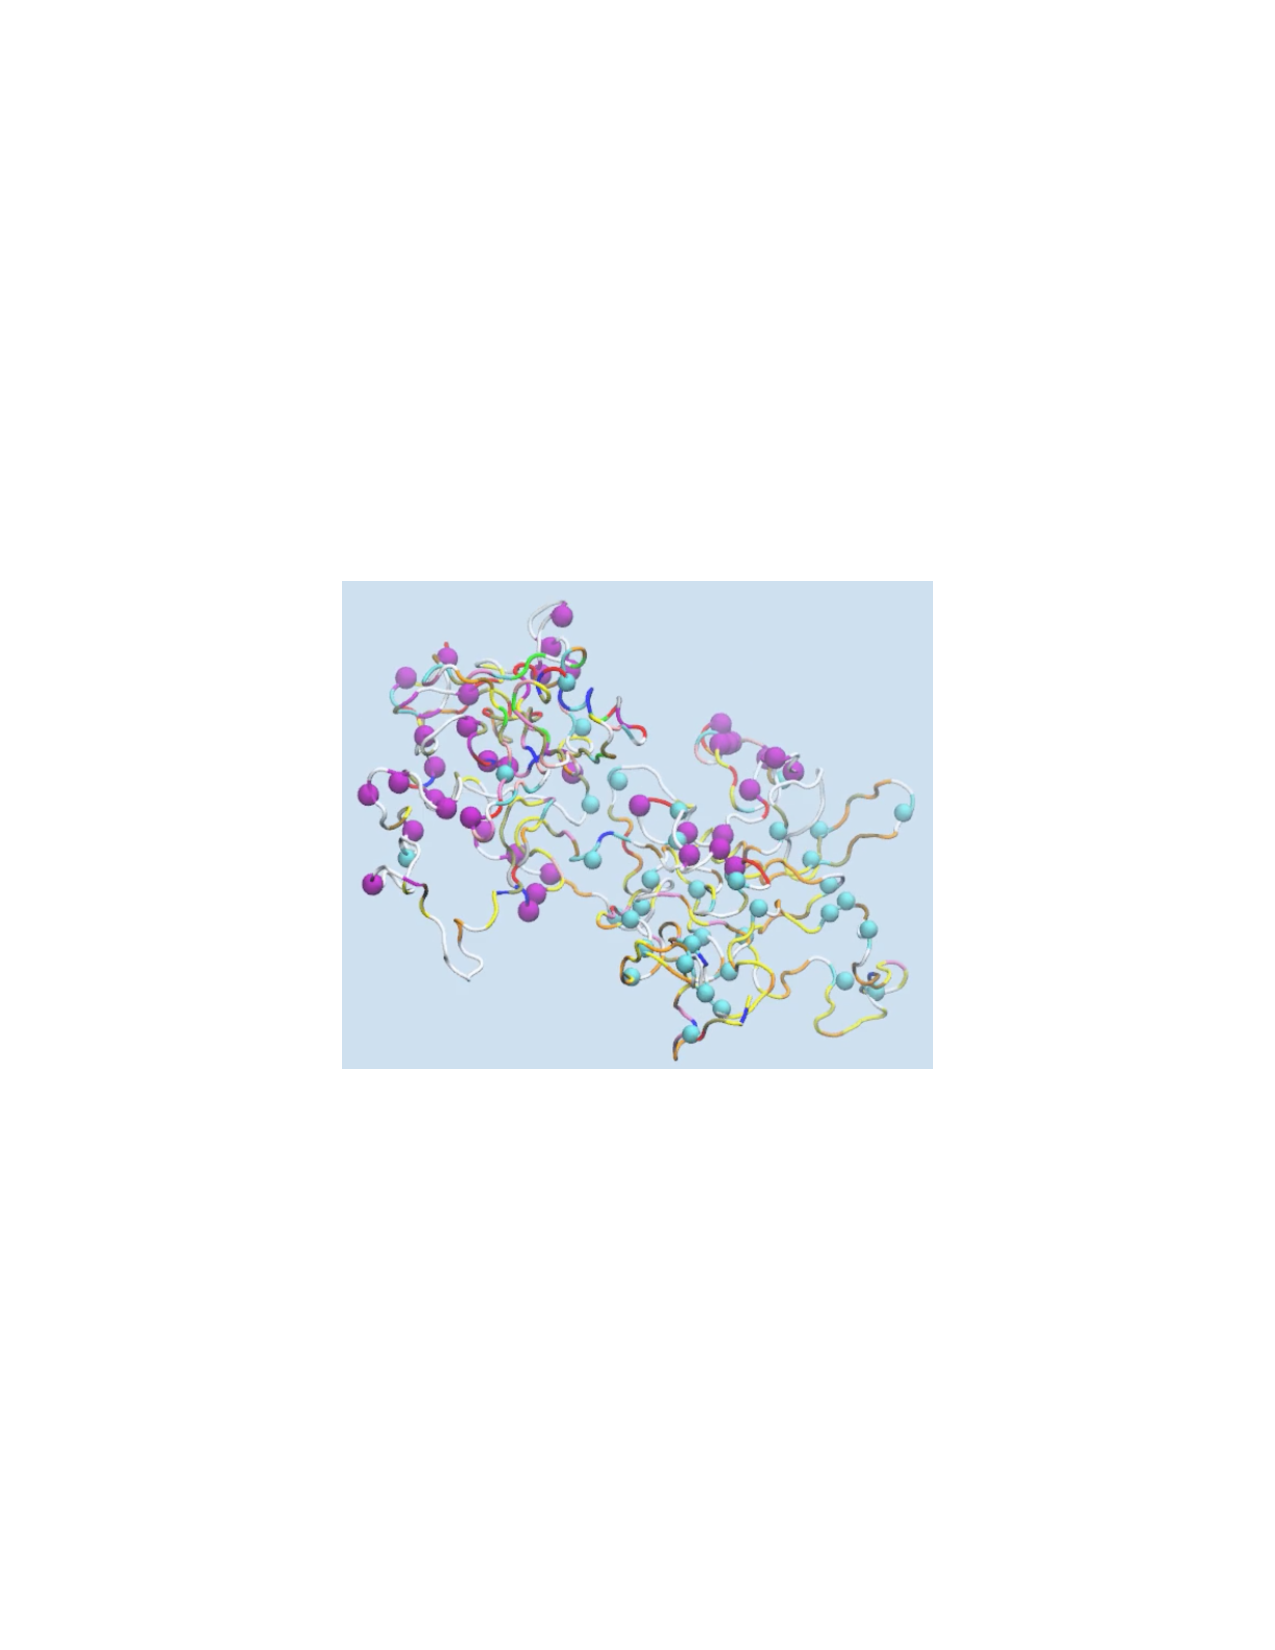
\includegraphics[width=5cm]{contact_fus.pdf} }}
    \caption {\small All-atom model of FUS in VDW representation}
    \label{fig:fus_430}
\end{figure}
\newpage

\section{Discussion}
The outcome of proteins, in this study FUS, undergoing liquid-liquid phase separation resembles liquid droplets, which is caused by the condensation into a dense phase \cite{Alberti_19}. LLPS is driven by the exchange of macromolecule/water interactions for macromolecule/macromolecule and water/water interactions under conditions for which this process is energetically favorable \cite{Alberti_19}. Therefore, the LLPS process is sensitive to environmental conditions such as temperature and concentration also plays an important role. \\[0.01cm]

To investigate the temperature-dependence on LLPS process of FUS, 10 simulations are run for a long period of time. The state of the system at the end of 8 $\mu s$ ARBD simulation run at $350K$ has formed what appears to be a cluster, a condensate as seen in Figure 2(b) above. In contrast, if we observe the system which was run at 430K, Figure 3(b), the proteins have not coalesced at all. Among the 10 simulations run at aforementioned temperatures, LLPS process occurs around $425K$ at x concentration. Each simulation took approximately 24 hrs to run when 1 unit of GPU is used for x concentration system. To understand how concentration affects the phase separation process, higher concentrations of x are continuing to be run at the same temperatures as well as lower ones. However, these simulations takes almost 3 times longer than the x concentration system so the results require more time. Given the duration of the internship and the availability of GPUs, it is difficult to simulate as many simulations necessary to achieve more results to quantify the phase separation phenomena. Even usage of supercomputers still have time constraints as there is a limit on how many node hours one job submission will get. \\[0.01cm] 

From previously published research study, we know that interactions between tyrosine and arginine residues are the principal drivers of LLPS. In Figure 4(b), the tyrosine residues are colored blue and arginine residues are colored purple, and Figure 4(a) shows the number of contacts between them over the $100$ ns all-atom simulation. 
  
\section{Conclusion}
The liquid-liquid phase separation process is very temperature and concentration dependent as at temperatures higher than $425K$, the proteins didn't coalesce. However, at room temperature or temperatures lower than $425K$, the phase separation occurs. Hence, the cut-off temperature for LLPS is at $425K$. 

\section{Future Directions}
More simulations at various concentration should be run to find out the cut-off concentration to case phase separation. Moreover, more simulations with mutant FUS needs to be run to gain insight into how certain mutations affect the phase separation process of FUS.
\newpage

\section{References}
\bibliography{ref_ncsa}
\bibliographystyle{plain}
%[1] A. Patel, et al. A Liquid-to-Solid Phase Transition of the ALS Protein FUS Accelerated by Disease Mutation. Cell. 2015. [done]
%[2] A. Mullard, Biomolecular Condensates Pique Drug Discovery curiosity. Nature Reviews Drug Discovery 18, 324-326, 2019 [done]
%[3] S. Banani, Biomolecular Condensates: organizers of cellular biochemistry. Nature Reviews Molecular Cell Biology, 18:285, 2017 [done]
%[4] H. Deng, The role of FUS gene variants in neurodegenerative diseases. Nature Reviews Neurology volume 10, pages 337–348 (2014) [done]
%[5] J. Mittal, Sequence determinants of protein phase behavior from a coarse-grained model. PLOS Computational Biology. [2018] [done]
%[6] J. Wang, et al. A molecular grammar governing the driving forces for phase separation of prion-like RNA binding proteins. Cell. 2018. [done]
%[7] D. T. Murray, et al. Structure of FUS protein fibrils and its relevance to self-assembly and phase separation of low-complexity domains. Cell, 171:615–627, 2017 [done]

\end{document}